\section{Disparate Risk}
\label{sec:disparate-risk}

Across every dataset we study, raw (pre-mechanism) re-identification
risk falls monotonically, or close to it, from the lowest- to the
highest-entropy decile: the least routine users are, unsurprisingly,
the hardest to re-identify to begin with (Figure~\ref{fig:raw-vs-post}).
The question this section asks is whether plain Mo-PAE's privacy
mechanism \emph{equalizes} that disparity, leaves it unchanged, or
widens it.

\begin{figure}[t]
\centering
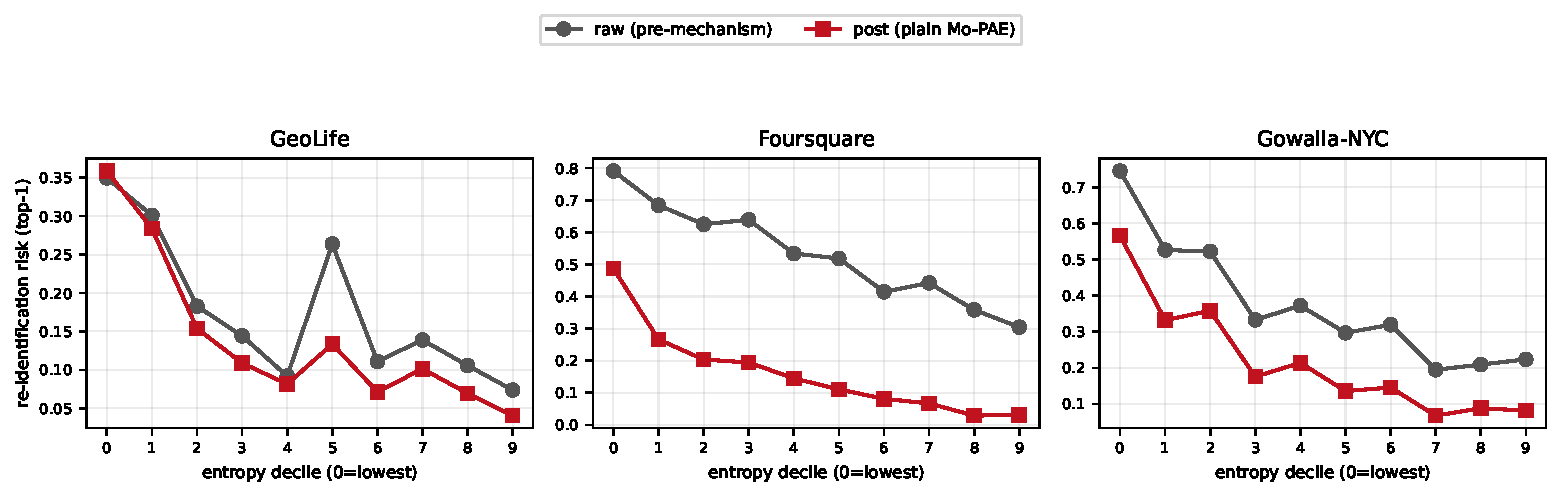
\includegraphics[width=\linewidth]{figures/fig1_raw_vs_post_by_decile.pdf}
\caption{Raw (pre-mechanism) vs.\ post-mechanism (plain Mo-PAE)
re-identification risk by entropy decile, GeoLife, Foursquare, and
Gowalla-NYC. The gap between the two lines narrows toward decile 0 in
every dataset: the most-identifiable decile keeps the largest share of
its original risk.}
\label{fig:raw-vs-post}
\end{figure}

On GeoLife and Foursquare, plain Mo-PAE reliably reduces risk for users
in the middle of the entropy distribution, but gives the lowest-entropy
decile no statistically detectable benefit beyond what a regression on
entropy, radius of gyration, and window count alone would predict --
entropy survives these controls as a significant negative predictor of
post-mechanism risk in every dataset we study (all $p < 10^{-6}$).
Table~\ref{tab:main-disparate-risk} reports the corrected decile-level
metrics (Section~\ref{sec:decile-reduction-metrics}) for these two
datasets plus Gowalla-NYC: on GeoLife, decile 0's relative risk
reduction is not statistically distinguishable from zero while decile
9's is; on Foursquare and Gowalla-NYC, decile 0 does receive a clearly
nonzero reduction, but far less than decile 9's, leaving a residual-risk
disparity ratio of 7--16$\times$ across the three datasets (every CI
excluding $1\times$, i.e.\ no disparity) and an absolute risk gap of
0.3--0.5 between the two deciles.

\begin{table*}[t]
\centering
\caption{Residual-risk disparity under plain Mo-PAE -- ratio (decile 0 $\div$ decile 9) and absolute difference (decile 0 $-$ decile 9) of post-mechanism risk -- and relative risk reduction at deciles 0 and 9, GeoLife, Foursquare, and Gowalla-NYC. Bootstrap 95\% CIs in brackets. Generated from \texttt{reports/figures/paper\_section8/geolife\_foursquare\_disparate\_risk.json}.}
\label{tab:main-disparate-risk}
\small
\begin{tabular}{@{}lccccc@{}}
\toprule
Dataset & $n$ & Rel.\ reduction, decile 0 & Rel.\ reduction, decile 9 & Disparity ratio (0/9) & Disparity difference (0$-$9) \\
\midrule
GeoLife & 178 & -0.032 [-0.189, +0.105] & +0.434 [+0.167, +0.617] & 8.81$\times$ [4.54, 15.16] & 0.318 [0.156, 0.495] \\
Foursquare & 1083 & +0.384 [+0.331, +0.439] & +0.897 [+0.866, +0.925] & 15.54$\times$ [10.84, 23.71] & 0.456 [0.396, 0.519] \\
Gowalla-NYC & 272 & +0.240 [+0.115, +0.371] & +0.634 [+0.519, +0.731] & 6.93$\times$ [4.24, 11.71] & 0.484 [0.336, 0.636] \\
\bottomrule
\end{tabular}
\end{table*}


Table~\ref{tab:gowalla-disparate-risk} reports the same metrics on all
four Gowalla metro subsets. In every one, the relative risk reduction
at the lowest-entropy decile is smaller than at the highest -- in
Gowalla-Chicago's smallest-sample case, the point estimate is slightly
negative, though its CI includes zero -- and the residual-risk
disparity ratio between the two deciles is large and statistically
significant in all four metros (2.2--5.9$\times$, every CI excluding
$1\times$).

\begin{table*}[t]
\centering
\caption{Residual-risk disparity (post-mechanism risk, decile 0 $\div$ decile 9) and relative reduction at deciles 0 and 9, plain Mo-PAE, all four Gowalla metro subsets. Bootstrap 95\% CIs in brackets. Generated from \texttt{reports/figures/phase2d/decile\_reduction\_metrics.json}.}
\label{tab:gowalla-disparate-risk}
\small
\begin{tabular}{@{}lccc@{}}
\toprule
Dataset & Rel.\ reduction, decile 0 & Rel.\ reduction, decile 9 & Residual disparity (0/9) \\
\midrule
Gowalla-NYC & 0.182 [0.116, 0.255] & 0.436 [0.328, 0.540] & 5.85$\times$ [3.87, 8.99] \\
Gowalla-LA & 0.183 [0.073, 0.321] & 0.477 [0.426, 0.529] & 2.23$\times$ [1.25, 3.46] \\
Gowalla-Chicago & -0.010 [-0.182, 0.140] & 0.450 [0.342, 0.547] & 5.40$\times$ [2.62, 9.75] \\
Gowalla-SF-Bay & 0.243 [0.159, 0.335] & 0.564 [0.513, 0.612] & 3.14$\times$ [2.19, 4.30] \\
\bottomrule
\end{tabular}
\end{table*}


A ratio and an absolute difference can disagree in direction whenever
both deciles' risk is falling but the higher-entropy decile's is
falling faster in relative terms -- Section~\ref{sec:residual-risk}
reports a case where this happens, and Table~\ref{tab:main-disparate-risk}
reports both statistics throughout this paper for exactly this reason.
